\section{Resultados}
% Eu sei precisa colocar a imagem ajustar a imagem, mas calma, não sufoca o artista

\subsection{Quantificação e pureza do DNA} A quantificação do DNA genômico foi
realizada por espectrofotometria utilizando equipamento NanoDrop, com análise
das razões de absorbância A\textsubscript{260}/A\textsubscript{280} e
A\textsubscript{260}/A\textsubscript{230}.  A amostra analisada apresentou
concentração de 140{,}1~ng/µL, com razão
A\textsubscript{260}/A\textsubscript{280} de 2{,}07 e
A\textsubscript{260}/A\textsubscript{230} de 2{,}31. Esses valores indicam alta
pureza, com ausência significativa de contaminantes como proteínas (razão
esperada entre 1{,}8 e 2{,}0) ou compostos orgânicos/sais (razão
A\textsubscript{260}/A\textsubscript{230} ideal > 1{,}8)\cite{Alguém}. A
qualidade do DNA obtido foi considerada adequada para as reações de PCR
subsequentes.

\subsection{Análise por PCR convencional} A identificação molecular da
amostra-problema foi conduzida por meio de três reações de PCR convencionais,
designadas como PCR-A, PCR-B e PCR-C, cada uma com especificidade crescente em
relação ao táxon de interesse. Os produtos amplificados foram analisados por
eletroforese em gel de agarose a 1{,}5\%, conforme apresentado nas
\cref{pcrA} e \cref{pcrBC}.

\begin{wrapfigure}{L}{.45\textwidth}
 \centering
 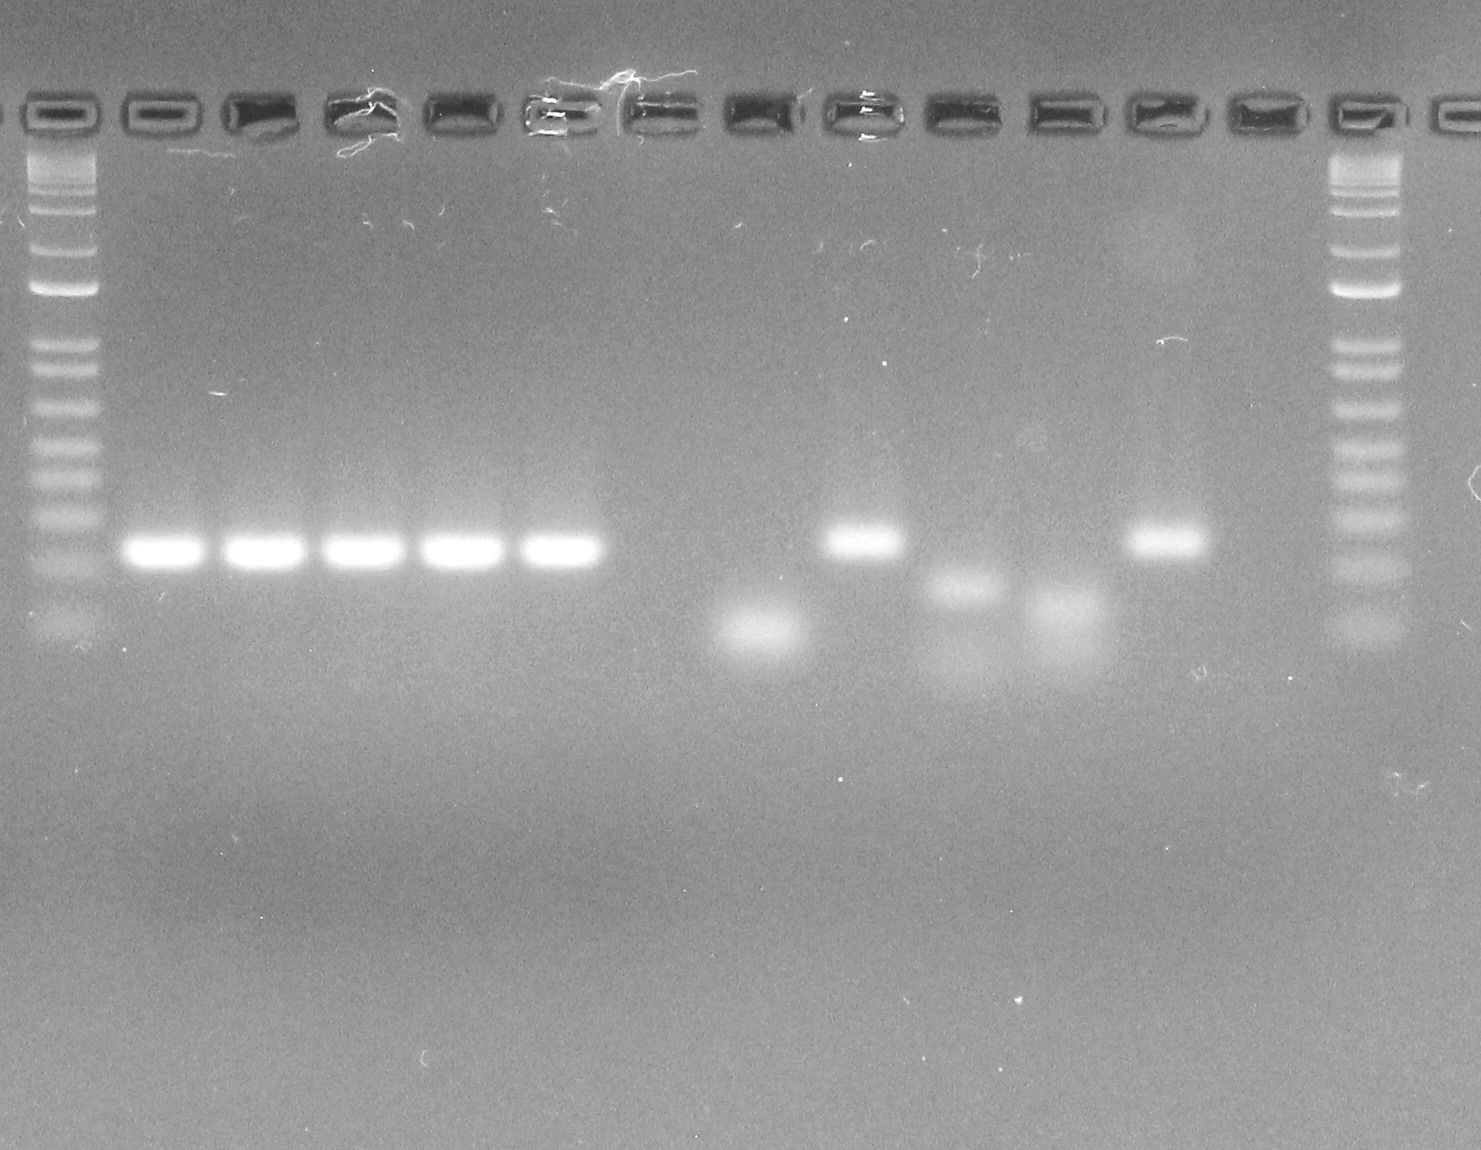
\includegraphics[width=.4\textwidth]{fig/pcrA_rflp_g8.jpg}
 \caption{Eletroforese dos produtos da PCR-A (gênero específico). As extremidades do gel contém escadas de peso molecular (ladders). 
 Os primeiros cinco poços da esquerda correspondem às amostras de DNA testadas quanto à presença do gênero \textit{Leishmania}, 
 seguidos por um controle negativo (água). Os poços subsequentes contêm, respectivamente: (1) \textit{L. (L.) infantum}, 
 (2) \textit{L. (L.) amazonensis}, (3) \textit{L. (V.) braziliensis}, (4) \textit{L. (V.) shawi}, (5) amostra-problema (W) e (6) controle negativo.}
 \label{pcrA}
 \end{wrapfigure}

A Figura~\ref{PCR_A} apresenta os resultados da eletroforese em gel de agarose referente à PCR-A, que tem como alvo uma região conservada do DNA genômico do gênero
 \textit{Leishmania}. Esta reação teve como objetivo inicial confirmar se a amostra-problema pertencia ao gênero, além de compará-la com amostras de referência previamente 
 caracterizadas.. Observa-se que tanto a amostra-problema (poço 5) quanto a amostra-controle de \textit{L. (L.) amazonensis} (poço 2) apresentaram bandas com o mesmo tamanho 
 molecular e intensidade semelhante. Esse padrão sugere fortemente que a amostra W pertence à mesma espécie ou, no mínimo, ao mesmo subgênero da amostra-controle. Por outro 
 lado, as demais amostras  exibiram perfis distintos, e os controles negativos (poços 6 e 12) não apresentaram amplificação, confirmando a ausência de contaminações cruzadas.
Esses dados sustentam a hipótese de que a amostra-problema pertence ao gênero \textit{Leishmania}, com forte indício de pertencimento à espécie \textit{L. (L.) amazonensis}, 
conforme indicado pela coincidência do perfil eletroforético com a amostra-controle correspondente.

\begin{wrapfigure}{R}{.45\textwidth}
 \centering
 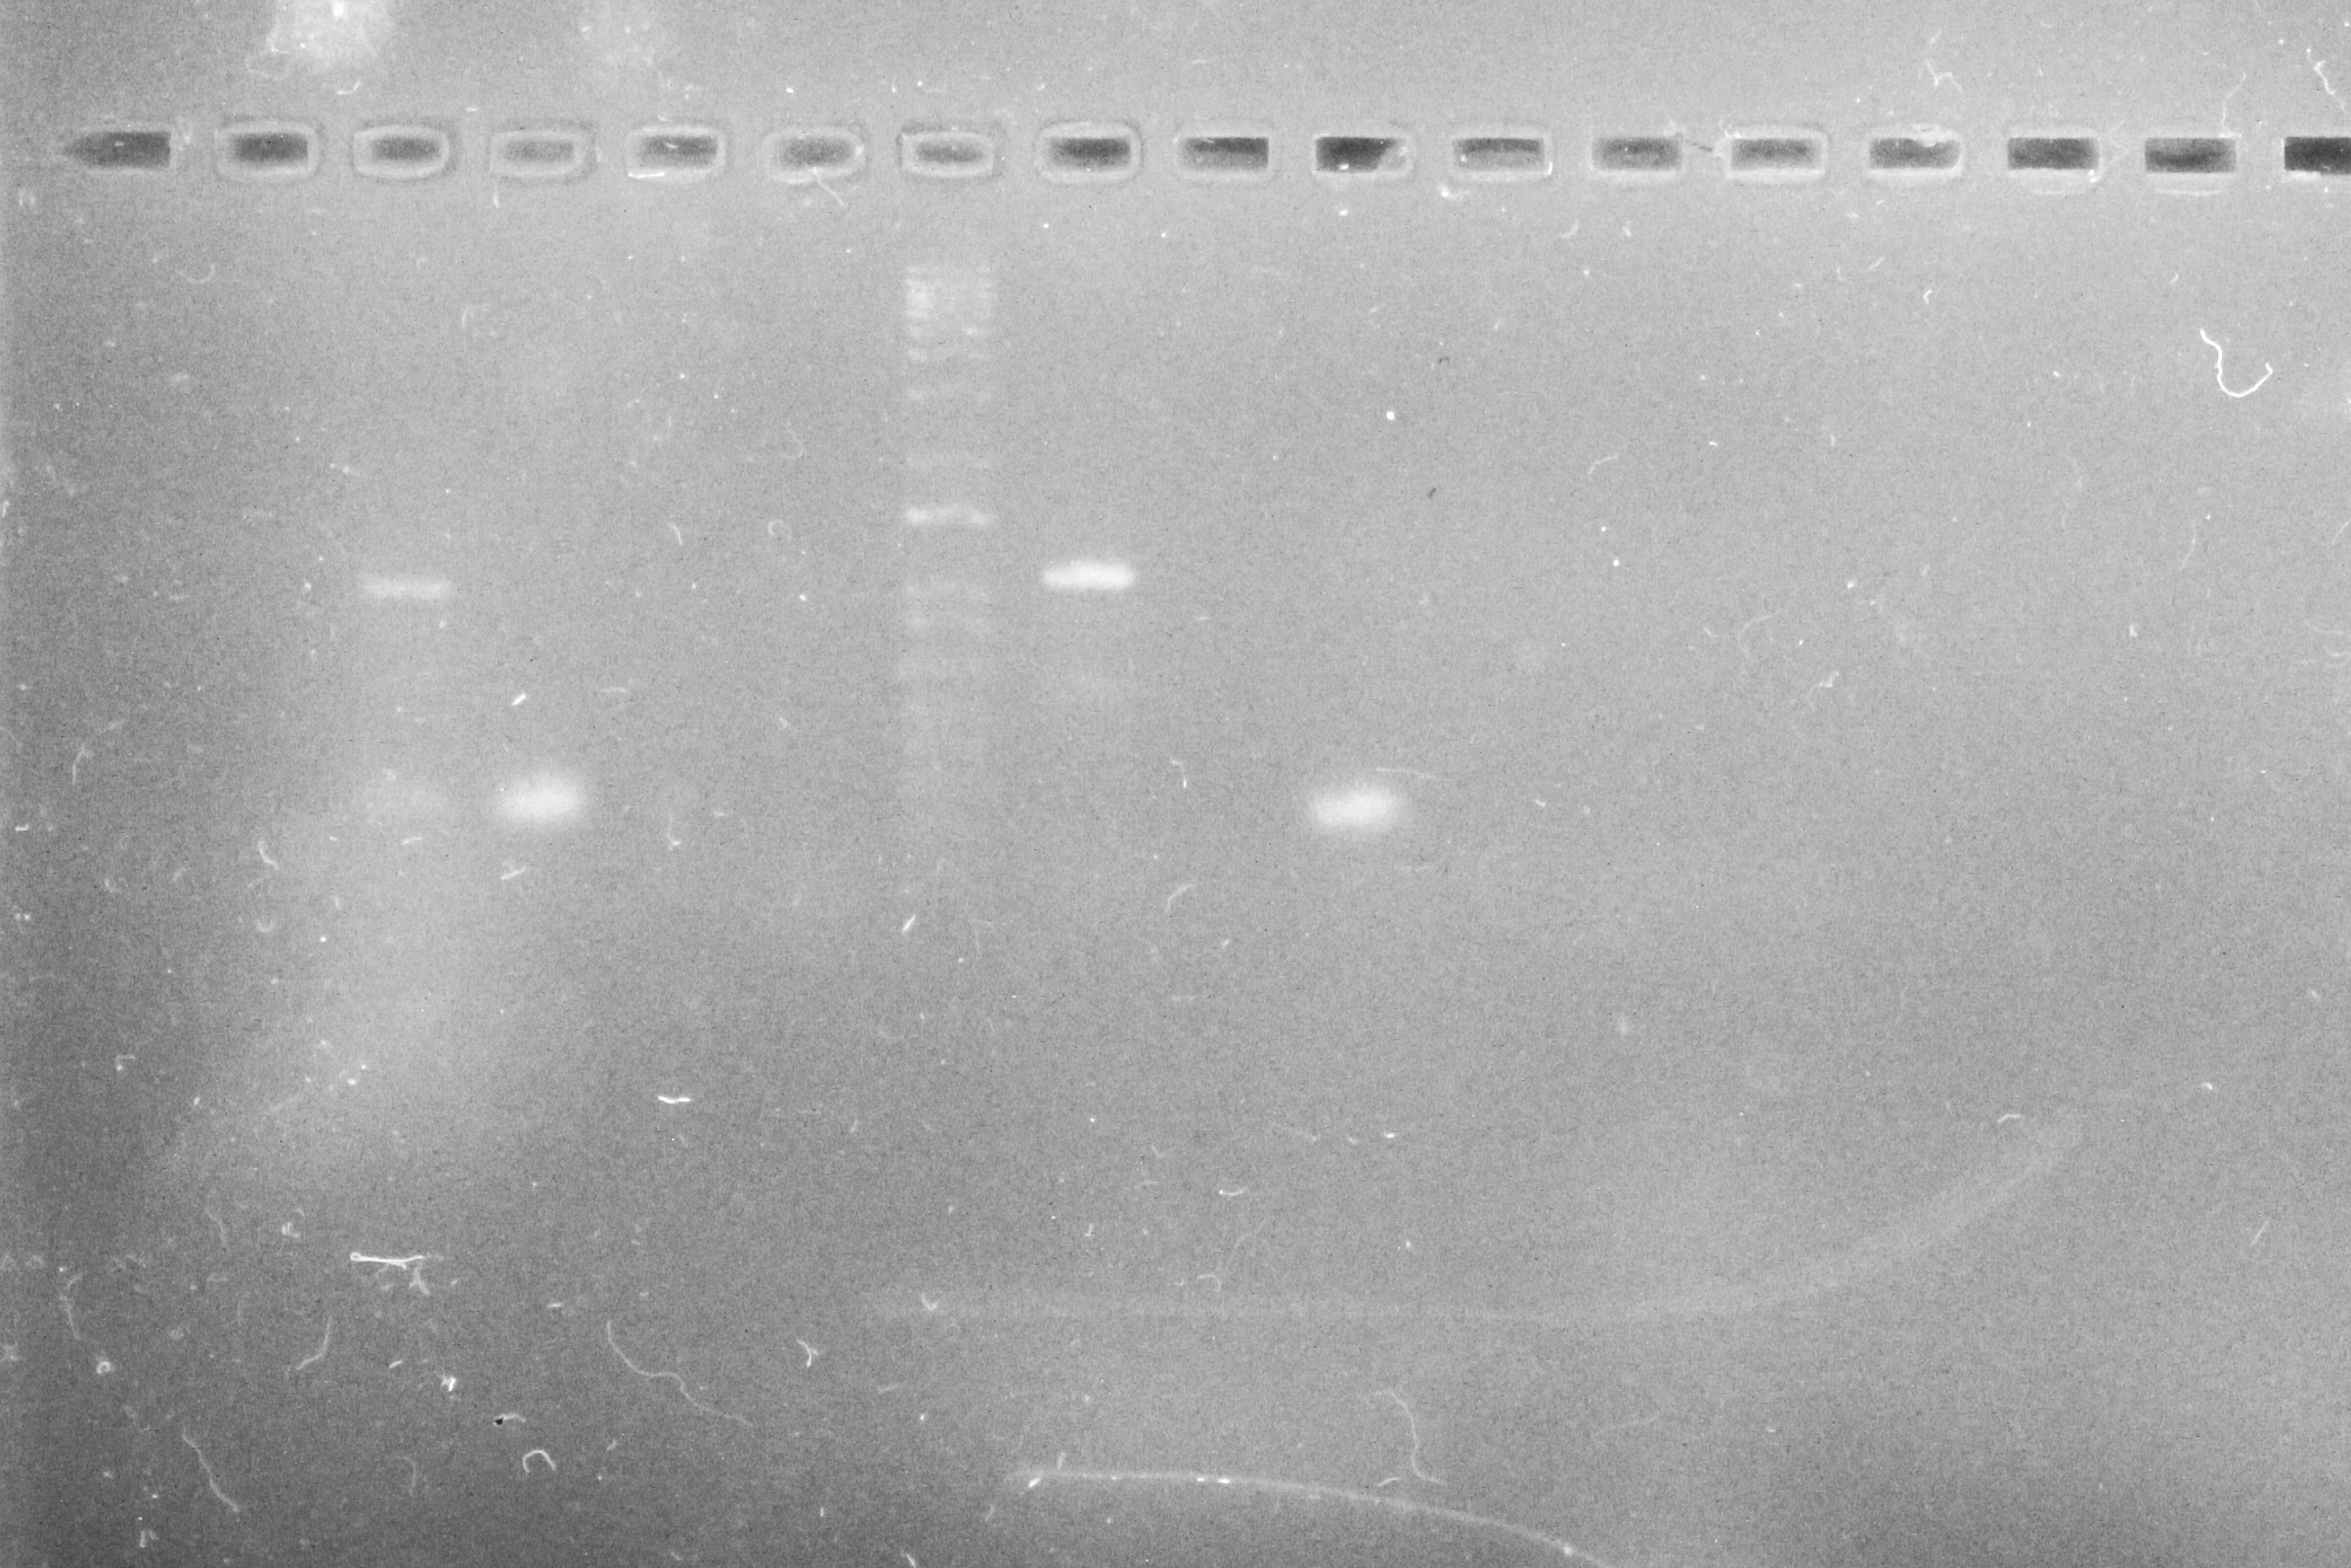
\includegraphics[width=.4\textwidth]{fig/pcrBeC_g8.jpg}
 \caption{Eletroforese dos produtos da PCR-B (subgênero \textit{Viannia}) e PCR-C (espécies não-\textit{braziliensis} do subgênero \textit{Viannia}). 
 A primeira série de seis poços à esquerda refere-se à PCR-B; em seguida há um poço com escada de peso molecular (ladder), seguido por seis poços referentes 
 à PCR-C. A ordem das amostras em ambas as reações é: (1) \textit{L. (L.) infantum}, (2) \textit{L. (L.) amazonensis}, (3) \textit{L. (V.) braziliensis}, 
 (4) \textit{L. (V.) shawi}, (5) amostra-problema (W) e (6) controle negativo.}
 \label{pcrBC}
 \end{wrapfigure}

As reações subsequentes, PCR-B e PCR-C, foram desenhadas com primers específicos para o subgênero \textit{Leishmania (Viannia)} e para espécies não-\textit{brasiliensis} dentro 
deste subgênero, respectivamente. Em ambas as reações, a amostra W não apresentou bandas detectáveis, ao contrário dos controles positivos específicos para \textit{L. (Viannia) 
braziliensis} e outras espécies do subgênero. A ausência de amplificação nas PCRs B e C reforça que a amostra W não pertence ao subgênero \textit{Viannia}, corroborando a classificação 
como \textit{Leishmania (Leishmania) amazonensis} já inferida pela PCR-A.

Na PCR-B, específica para o subgênero não-\textit{Leishmania (Viannia)}, foi observada uma banda nítida no poço 4, correspondente à amostra \textit{L. (V.) shawi}, como esperado. 
No entanto, uma banda mais tênue e não prevista foi detectada no poço 3, referente a \textit{L. (V.) braziliensis}, o que pode indicar uma amplificação inespecífica ou contaminação 
pontual. As demais amostras, incluindo a amostra-problema (poço 5), não apresentaram bandas visíveis, sugerindo ausência de amplificação com os primers utilizados nesta reação.

Já na PCR-C, voltada à detecção de espécies \textit{braziliensis} dentro do subgênero \textit{Viannia}, foi identificada uma banda clara no poço 3 (L. (V.) braziliensis}), 
como previsto. No entanto, uma amplificação não esperada foi observada no poço 1, correspondente a \textit{L. (L.) infantum}, o que sugere a possibilidade de reação cruzada ou mínima 
contaminação da amostra.

\subsection{Análise da amplificação e \textit{melting temperature} obtidos por
qPCR e HRM}

As curvas de \textit{melting} foram obtidas com o software High
Resolution Melt v.3.0.1 (Life Technologies) com resolução de
\qty{0,2}{\celsius}, após a amplificação por PCR em tempo real.

\begin{figure}[b!]
        \centering
        \includegraphics[width=.9\textwidth]{fig/paduni_prancheta_v2}
        \caption{Curvas de \textit{melting} obtidas por qPCR acoplado à HRM dos amplicons de \textit{L. (L.)
        amazonensis} (em laranja), \textit{L. (V.) braziliensis} (em roxo),
    \textit{L. (L.) infantum} (em vermelho) e \textit{L. (V.) shawi} (em rosa).
A \textit{Derivative melt curve} em A evidência as Tm de cada espécie. Em B
vê-se as curvas alinhadas evidenciando o perfil de \textit{melting}.}
        \label{paduni}
\end{figure} 

As amostras conhecidas, tiveram seu perfil de \textit{melting} determinado por
Zampieri et.al.\cite{HRMzampi2016}. O perfil obtido está resumino na
\cref{paduni}.  É possível observar a \textit{melting temperature} (Tm) de cada
espécie nas curvas derivadas da fluorescência em função da temperatura
(derivative melt curves) \cref{paduni}A.

As diferenças entre os perfis de \textit{melting} das amostras são evidenciadas
nas curvas de diferença (\cref{paduni}B).  É notável que cada espécie estudada
apresentou comportamento de \textit{melting} único em comparação às demais.
Essas diferenças são exatamente conforme o esperado de acordo com o trabalho de
Zampieri et.al.\cite{HRMzampi2016} e são decorrentes de pequenas diferenças nas
sequências dos amplicons de cada espécie.

Ainda, é possível observar o padrão das amostras com \textit{L. (V.) shawi} e
\textit{L. (V.) brasilienses} que são visualmente distinguíveis na
\cref{paduni}B. Já as curvas de \textit{L. (L.) amazonensis} e \textit{L. (L.)
infantum} são mais similares entre si, embora facilmente distinguível das outras
duas,  com a maior diferença observável em valores pouco menores à
\qty{87}{\celsius}.

\begin{figure}[b!]
        \centering
        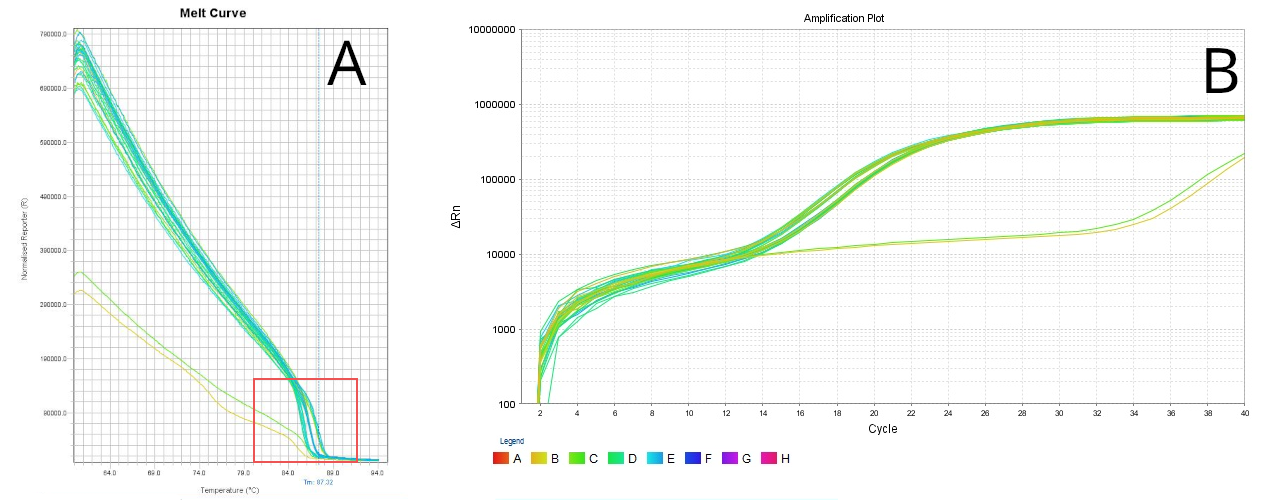
\includegraphics[width=.9\textwidth]{fig/prancheta_test_PCR}
        \caption{Perfil de \textit{melting} (A) e amplificação (B) obtidos por
            qPCR acoplada à HRM da placa com amostras de controle positivo de \textit{L. (L.)
        amazonensis}, \textit{L. (V.) braziliensis},
    \textit{L. (L.) infantum} e \textit{L. (V.) shawi} e controle negativo nas
    curvas B (em amarelo) e C (em verde) e amostras desconhecidas W, X, Y, Z nas
    curvas D (em azul esverdeado) e E (em azul). O quadrado em vermelho em A
    marca a região em que o perfil de \textit{melting} é distinguível e
    comparável com os padrões.
}
        \label{tstuni}
\end{figure}

A reação de qPCR realizada originou a \cref{tstuni}, realizada com um conjunto
de amostras desconhecidas acompanhadas de controles positivos e negativos. A
curva de \textit{melting} (\cref{tstuni}A) revela que a maioria das amostras
desconhecidas apresenta perfis de \textit{melting} compatíveis com os observados
nas amostras padronizadas.

Como esperado, duas curvas presentes na reação de qPCR realizada exibem perfis
atípicos do padrão observado nas curvas com as amostras conhecidas, estas duas
curvas são referentes aos dois poços com controle negativo na placa. Isto é
corroborado ao avaliar as mesmas curvas na \cref{tstuni}B, que mostra as curvas
de amplificação correspondentes à mesma placa, em que esses dois poços não
apresentaram aumento significativo na fluorescência, comportamento compatível
com o esperado para os controles negativos incluídos na reação.

Ademais, na região de \qty{85}{\celsius}-\qty{88}{\celsius} da \cref{tstuni}A é
possível observar três padrões evidentemente diferentes e mais um que se
diferencia à pouco menos que \qty{87}{\celsius}. Estes são os mesmos quatro
padrões observados nas amostras conhecidas (\cref{tstuni}A).
